\documentclass{article}
\usepackage {graphicx}
%\bibliographystyle{apj}
\usepackage{graphics}
\title{Galaxy completeness in two massive fiber allocation setups}
\begin{document}
\maketitle
\section{Introduction}

\section{Fibers and Galaxies}

\subsection{Fibers}

\begin{figure}
\begin{center}
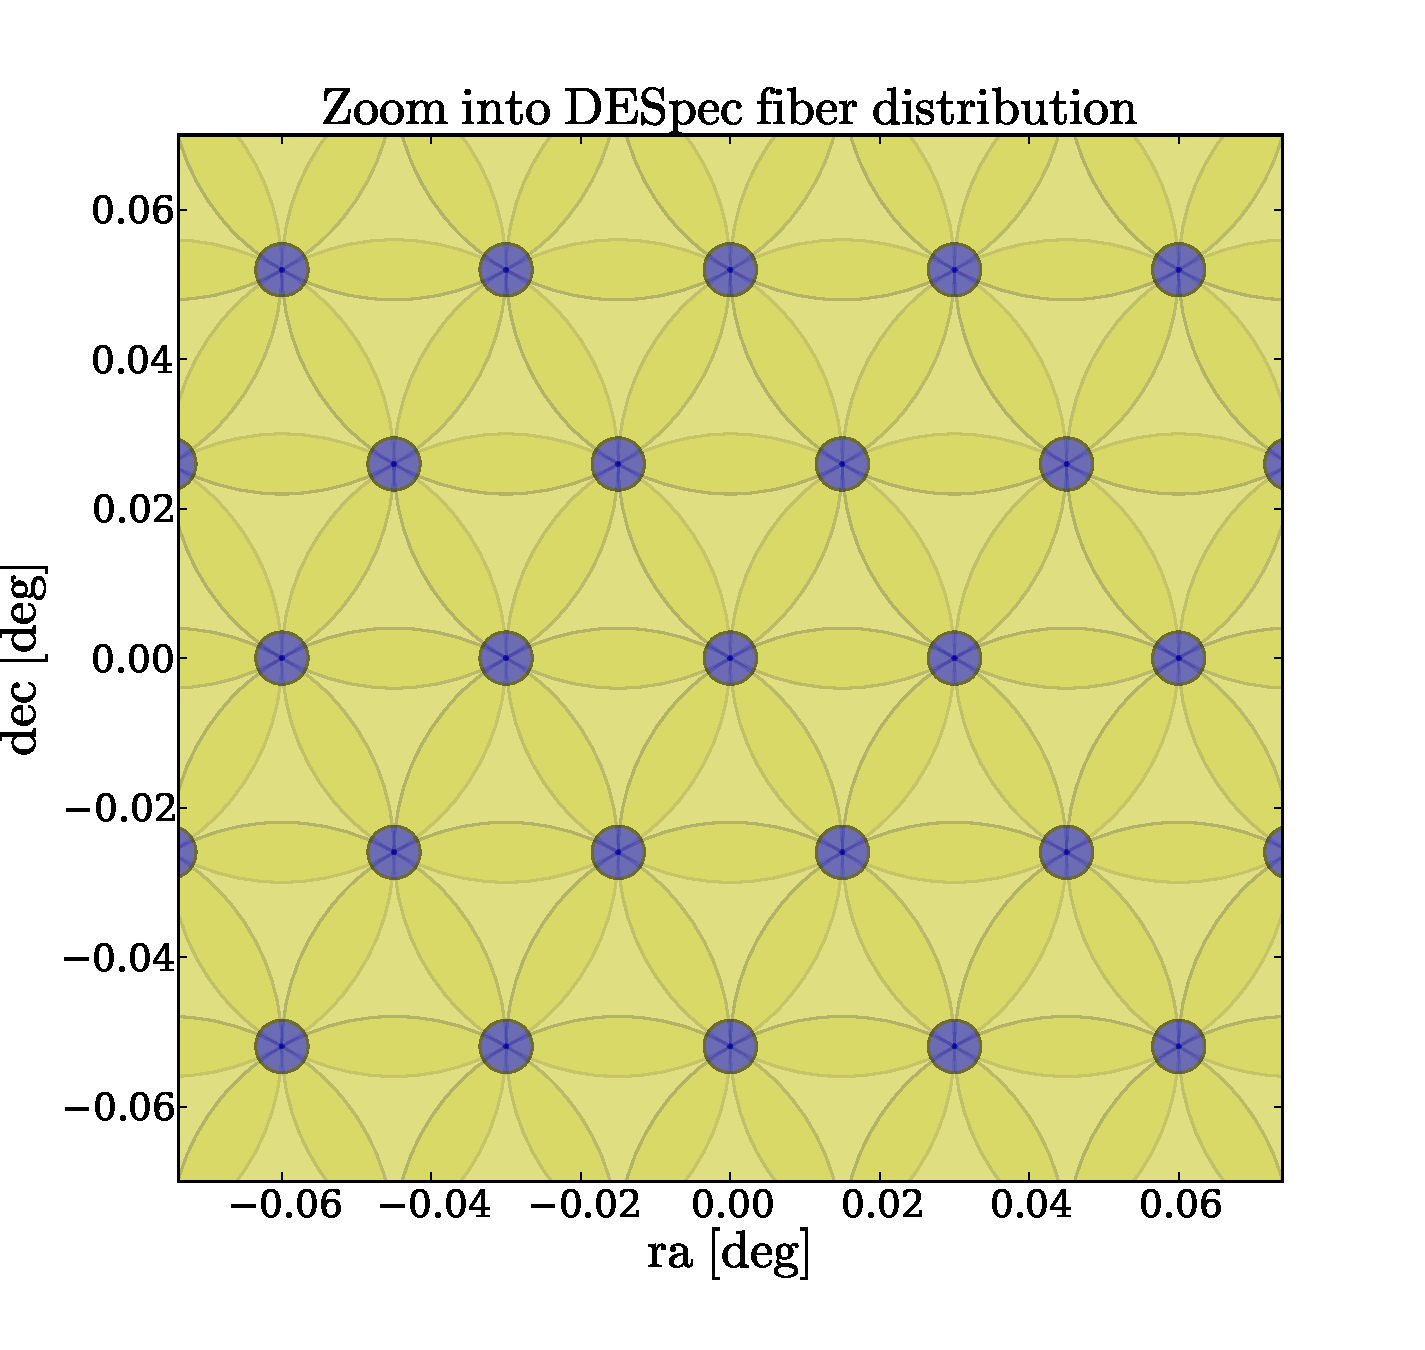
\includegraphics[keepaspectratio=true,width=0.7\textwidth]{DES_fibers_zoom.pdf}
\caption{Fiber distribution}
\end{center}
\end{figure}

\begin{figure}
\begin{center}
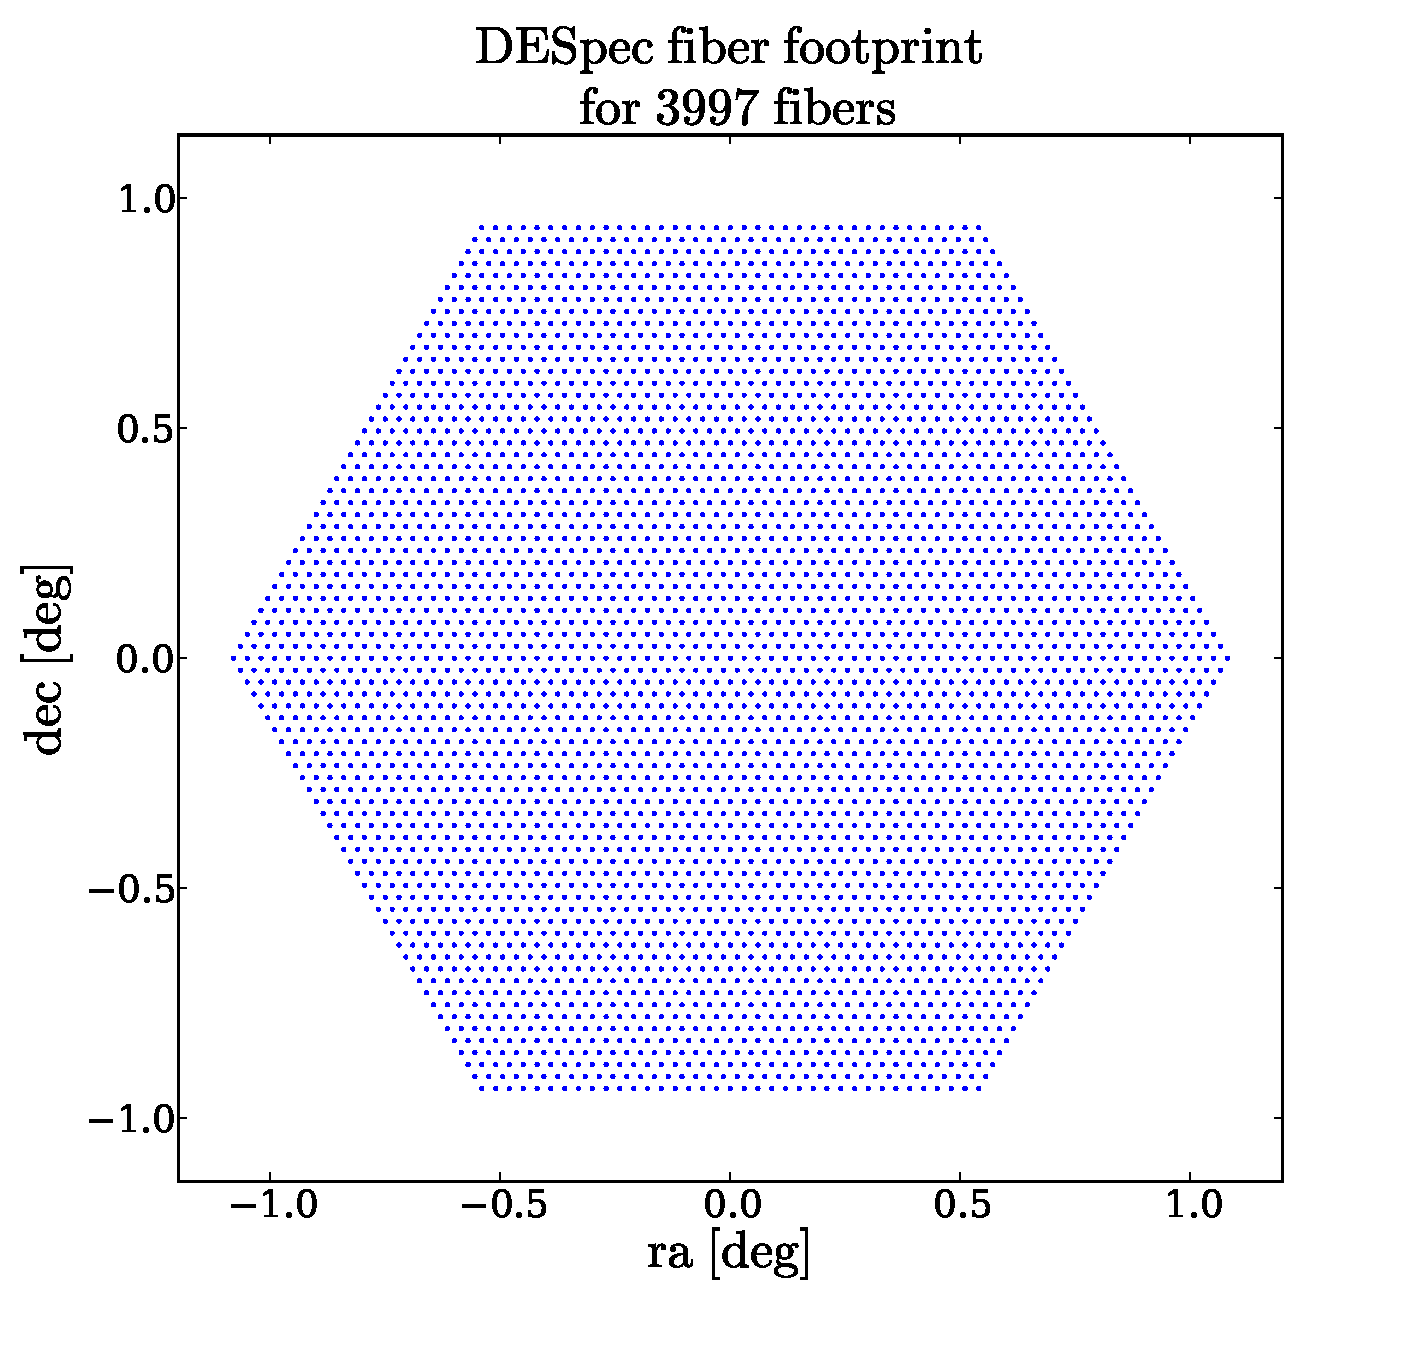
\includegraphics[keepaspectratio=true,width=0.7\textwidth]{DES_fibers.pdf}
\caption{Zoom into the Fiber distribution}
\end{center}
\end{figure}

\begin{figure}
\begin{center}
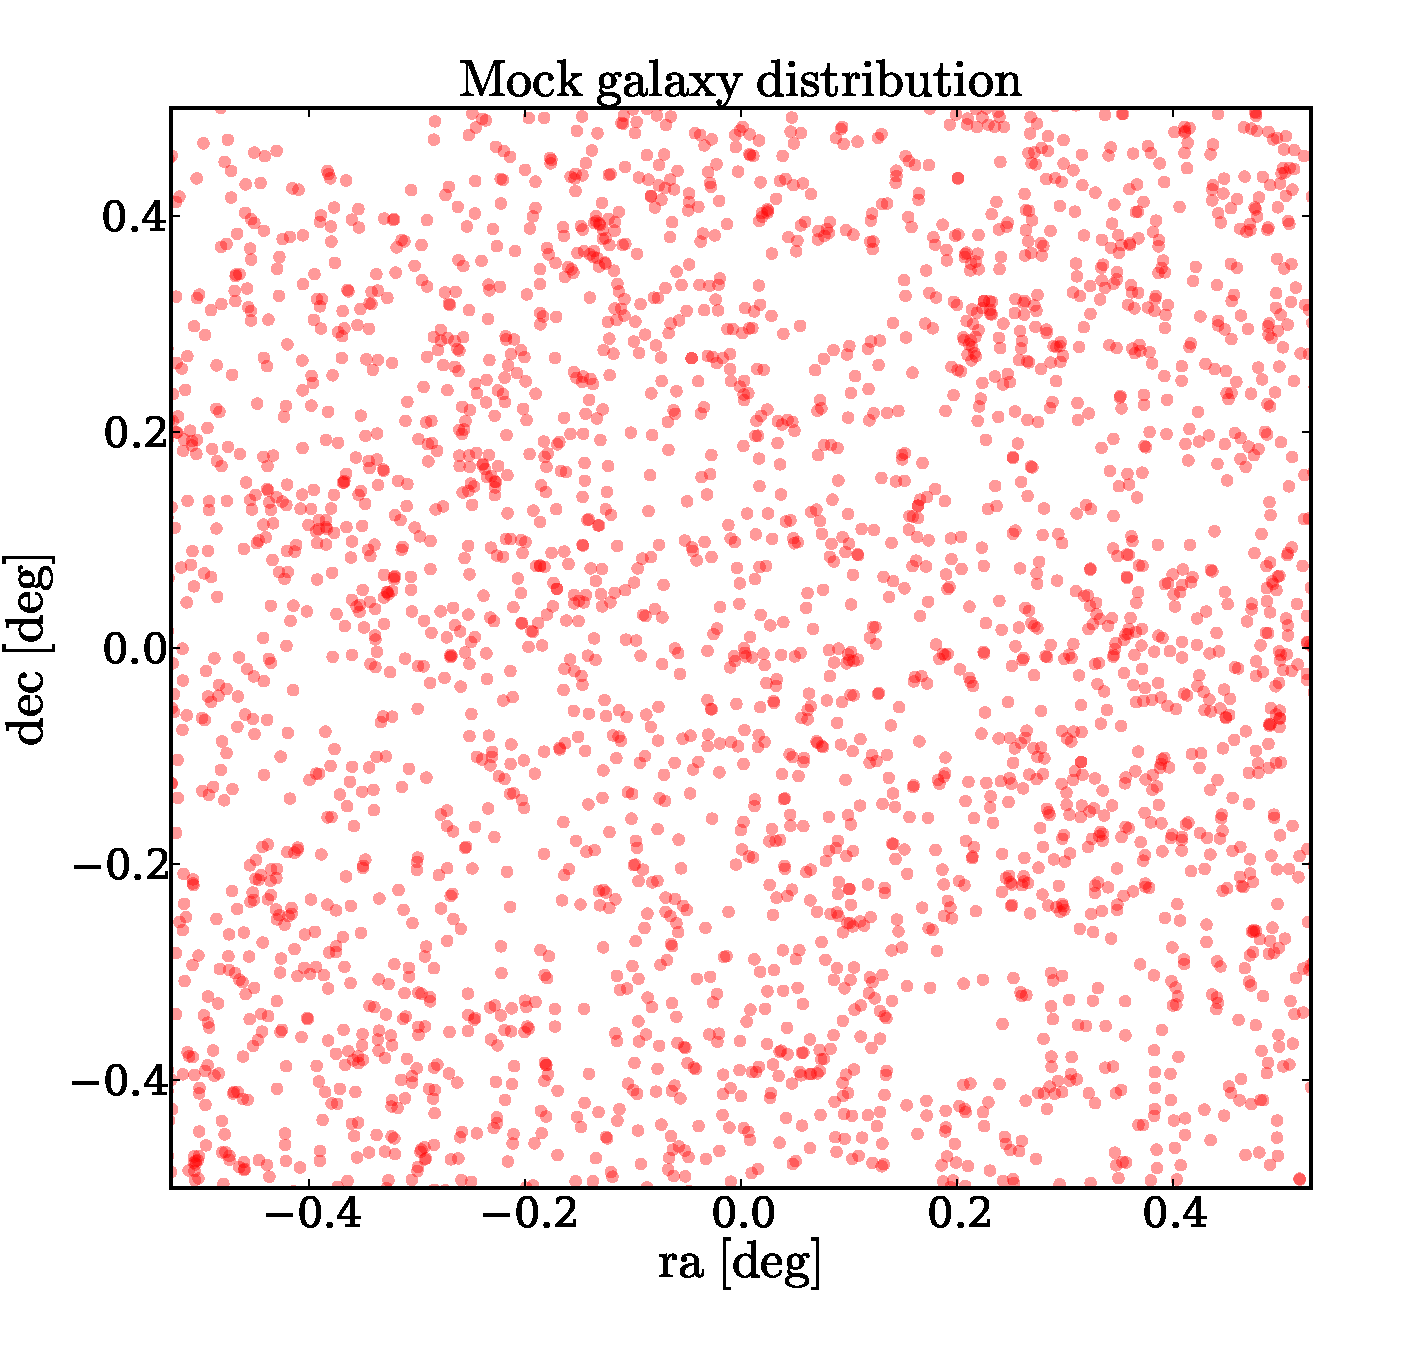
\includegraphics[keepaspectratio=true,width=0.7\textwidth]{mock_gals.pdf}
\caption{Galaxy distribution}
\end{center}
\end{figure}

The fibers are placed in an hexagonal tile following a pattern where
the inter-fiber distance, the pitch $P$, is the same for all
fibers. The pattern is shown in Figure 1. 

Each fiber tile is completely described by the patrol radius $r_{\rm
  p}$ and the exclusion radius $r_{\rm e}$.


We try to different setups the 
\begin{itemize}
\item {\rm Despec}. Patrol radius $r_{\rm p}=P$. Exclusion radius
  $r_{\rm e}=1/10\times P$
\item {\rm BB}. Patrol radius $r_{\rm p}=P/\sqrt{3}$. Exclusion radius
  $r_{\rm e}=0.15 \times P$
\end{itemize}

\subsection{Galaxies}
We use two kinds of galaxy distributions: poissonian and clustered. \\ 

The clustered simulations are built directly from the observed
COSMOS catalog of Capak et al. 2008, Ilbert et al. 2009. We refer to this simulation as the
COSMOS Mock Catalog (CMC) (Jouvel et al. 2009).
The COSMOS photometric-redshift catalog (Ilbert et al. 2009) was computed with 30 bands over 2 deg2
with data from GALEX, Subaru, CFHT, UKIRT, and Spitzer.
It achieves very good photo-z accuracy and low catastrophic redshift rates.
The CMC is restricted to the area fully covered by
HST/ACS imaging, 1.24 deg2 after removal of masked areas. There are a total of 538,000 simulated
galaxies at $i<26.5$, with a density of roughly 120 gal/arcmin2.
AGN, stars, and X-ray sources were removed from the input COSMOS catalog.
Using the best fit photo-z and template, we first produce simulated magnitudes
using DES filter transmission.
We then apply random errors to the simulated magnitudes based on a simple magnitude-error
relation in each filter. The simulated mix of galaxy populations is then, by construction,
representative of the COSMOS survey as well as the clustering and additional quantities measured in COSMOS such as
galaxy size, UV luminosity, morphology, stellar masses.
The CMC is limited to the range of magnitude
where the COSMOS imaging is complete $i_{AB} \approx 26.2$ for a 5 $\sigma$ detection (Capak et al. 2007 and 2008).
We associate emission-line fluxes for each galaxy of the CMC. We model the [OII] emission-line
using the Kennicutt 1998 calibration for restframe UV-[OII] emission-line flux relation.
For the other emission lines, we adopt intrinsic,
unextincted flux ratios of [OIII]/[OII] = 0.36; H beta/[OII] = 0.28; H alpha/[OII] = 1.77
and Ly alpha/[OII] = 2 (McCall 1985 Moustakas 2006, Kennicutt 2006, Mouhcine 2005, Kennicutt 1998).
It shows a good agreement with the VVDS observations
and is valid for the different galaxy population.
The CMC does an excellent job of reproducing the counts and color distributions of galaxies observed
in bands from 0.4 to 2.2 microns, when comparing to the GOODS (Giavalisco et al. 2004) and
UDF (Coe et al. 2006) surveys. The CMC also provides an excellent match to the redshift-magnitude
and redshift-color distributions for I$<$24 galaxies in the VVDS spectroscopic redshift survey (Le Fevre et al. 2005).
For more detail about the CMC and its validation, see Jouvel et al. 2009.

We used 2 types of targets: Emission-Line Galaxies(ELG) and Lyman Red Galaxies (LRG).
These galaxy types give the best probability of having a high spectroscopic success rate.
Using the CMC, we use simple criterion to do the target selection:\\
{$\bullet$} ELG: galaxies with at least 1 line at 5 sigma and a photoz selection to select highest redshift galaxies.\\
{$\bullet$} LRG: $S/N_{continuum}>2$ and a $photo-z>0.5$. 

\section{Allocation Algorithms}

We use two allocation algorithms

\subsection{Simulated Annealing}
...Simulated Annealing (SA)

\subsection{Local Galaxy Density}
...Local Galaxy Density (LGD)

\section{Results}

The following table summarizes our results

\begin{table}
\begin{tabular}{cccccc}\hline
Fiber & Galaxy & Allocation & \% Total & \% ELG & \% LRG\\
Setup & Distribution & Algorithm & Completeness & Completeness& Completeness\\\hline
DESpec & Poisson & SA & & -& -\\
BB & Poisson & SA & & -& -\\
DESpec & Mock & SA & & &\\
BB & Mock & SA & & &\\
DESpec & Poisson & LGD & 94 & -& -\\
BB & Poisson & LGD & 88& -&-\\
DESpec & Mock & LGD & 90 & 94 & 86\\
BB & Mock & LGD & & &\\\hline
\end{tabular}
\label{Summary of the results.}
\end{table}

\end{document}

